%
\begin{isabellebody}%
\setisabellecontext{StutteringDefs}%
%
\isadelimdocument
%
\endisadelimdocument
%
\isatagdocument
%
\isamarkupchapter{Properties of TESL%
}
\isamarkuptrue%
%
\isamarkupsection{Stuttering Invariance%
}
\isamarkuptrue%
%
\endisatagdocument
{\isafolddocument}%
%
\isadelimdocument
%
\endisadelimdocument
%
\isadelimtheory
%
\endisadelimtheory
%
\isatagtheory
\isacommand{theory}\isamarkupfalse%
\ StutteringDefs\isanewline
\isanewline
\isakeyword{imports}\ Denotational\isanewline
\isanewline
\isakeyword{begin}%
\endisatagtheory
{\isafoldtheory}%
%
\isadelimtheory
%
\endisadelimtheory
%
\begin{isamarkuptext}%
When composing systems into more complex systems, it may happen that one system 
  has to perform some action while the rest of the complex system does nothing.
  In order to support the composition of TESL specifications, we want to be able 
  to insert stuttering instants in a run without breaking the conformance of a run 
  to its specification. This is what we call the \emph{stuttering invariance} of TESL.%
\end{isamarkuptext}\isamarkuptrue%
%
\isadelimdocument
%
\endisadelimdocument
%
\isatagdocument
%
\isamarkupsubsection{Definition of stuttering%
}
\isamarkuptrue%
%
\endisatagdocument
{\isafolddocument}%
%
\isadelimdocument
%
\endisadelimdocument
%
\begin{isamarkuptext}%
We consider stuttering as the insertion of empty instants (instants at which no 
clock ticks) in a run. We caracterize this insertion with a dilating function,
which maps the instant indices of the original run to the corresponding instant
indices of the dilated run.
The properties of a dilating function are:

%
\begin{itemize}%
\item it is strictly increasing because instants are inserted into the run,

\item the image of an instant index is greater than it because stuttering instants 
can only delay the original instants of the run, 

\item no instant is inserted before the first one in order to have a well defined 
initial date on each clock,

\item if \isa{n} is not in the image of the function, no clock ticks at 
instant \isa{n} and the date on the clocks do not change.%
\end{itemize}%
\end{isamarkuptext}\isamarkuptrue%
\isacommand{definition}\isamarkupfalse%
\ dilating{\isacharunderscore}fun\isanewline
\isakeyword{where}\isanewline
\ \ {\isacartoucheopen}dilating{\isacharunderscore}fun\ {\isacharparenleft}f{\isacharcolon}{\isacharcolon}nat\ {\isasymRightarrow}\ nat{\isacharparenright}\ {\isacharparenleft}r{\isacharcolon}{\isacharcolon}{\isacharprime}a{\isacharcolon}{\isacharcolon}linordered{\isacharunderscore}field\ run{\isacharparenright}\isanewline
\ \ \ \ {\isasymequiv}\ strict{\isacharunderscore}mono\ f\ {\isasymand}\ {\isacharparenleft}f\ {\isadigit{0}}\ {\isacharequal}\ {\isadigit{0}}{\isacharparenright}\ {\isasymand}\ {\isacharparenleft}{\isasymforall}n{\isachardot}\ f\ n\ {\isasymge}\ n\isanewline
\ \ \ \ {\isasymand}\ {\isacharparenleft}{\isacharparenleft}{\isasymnexists}n\isactrlsub {\isadigit{0}}{\isachardot}\ f\ n\isactrlsub {\isadigit{0}}\ {\isacharequal}\ n{\isacharparenright}\ {\isasymlongrightarrow}\ {\isacharparenleft}{\isasymforall}c{\isachardot}\ {\isasymnot}{\isacharparenleft}ticks\ {\isacharparenleft}{\isacharparenleft}Rep{\isacharunderscore}run\ r{\isacharparenright}\ n\ c{\isacharparenright}{\isacharparenright}{\isacharparenright}{\isacharparenright}\isanewline
\ \ \ \ {\isasymand}\ {\isacharparenleft}{\isacharparenleft}{\isasymnexists}n\isactrlsub {\isadigit{0}}{\isachardot}\ f\ n\isactrlsub {\isadigit{0}}\ {\isacharequal}\ {\isacharparenleft}Suc\ n{\isacharparenright}{\isacharparenright}\ {\isasymlongrightarrow}\ {\isacharparenleft}{\isasymforall}c{\isachardot}\ time\ {\isacharparenleft}{\isacharparenleft}Rep{\isacharunderscore}run\ r{\isacharparenright}\ {\isacharparenleft}Suc\ n{\isacharparenright}\ c{\isacharparenright}\isanewline
\ \ \ \ \ \ \ \ \ \ \ \ \ \ \ \ \ \ \ \ \ \ \ \ \ \ \ \ \ \ \ \ \ \ \ \ \ \ {\isacharequal}\ time\ {\isacharparenleft}{\isacharparenleft}Rep{\isacharunderscore}run\ r{\isacharparenright}\ n\ c{\isacharparenright}{\isacharparenright}{\isacharparenright}\isanewline
\ \ \ {\isacharparenright}{\isacartoucheclose}%
\begin{isamarkuptext}%
A run \isa{r} is a dilation of a run \isa{sub} by 
function \isa{f} if:

%
\begin{itemize}%
\item \isa{f} is a dilating function for \isa{r} 

\item the time in \isa{r} is the time in \isa{sub} dilated by \isa{f}

\item the ticks in \isa{r} is the ticks in sub dilated by \isa{f}%
\end{itemize}%
\end{isamarkuptext}\isamarkuptrue%
\isacommand{definition}\isamarkupfalse%
\ dilating\isanewline
\isakeyword{where}\isanewline
\ \ {\isacartoucheopen}dilating\ f\ sub\ r\ {\isasymequiv}\ dilating{\isacharunderscore}fun\ f\ r\isanewline
\ \ \ \ \ \ \ \ \ \ \ \ \ \ \ \ \ \ \ \ {\isasymand}\ {\isacharparenleft}{\isasymforall}n\ c{\isachardot}\ time\ {\isacharparenleft}{\isacharparenleft}Rep{\isacharunderscore}run\ sub{\isacharparenright}\ n\ c{\isacharparenright}\ {\isacharequal}\ time\ {\isacharparenleft}{\isacharparenleft}Rep{\isacharunderscore}run\ r{\isacharparenright}\ {\isacharparenleft}f\ n{\isacharparenright}\ c{\isacharparenright}{\isacharparenright}\isanewline
\ \ \ \ \ \ \ \ \ \ \ \ \ \ \ \ \ \ \ \ {\isasymand}\ {\isacharparenleft}{\isasymforall}n\ c{\isachardot}\ ticks\ {\isacharparenleft}{\isacharparenleft}Rep{\isacharunderscore}run\ sub{\isacharparenright}\ n\ c{\isacharparenright}\ {\isacharequal}\ ticks\ {\isacharparenleft}{\isacharparenleft}Rep{\isacharunderscore}run\ r{\isacharparenright}\ {\isacharparenleft}f\ n{\isacharparenright}\ c{\isacharparenright}{\isacharparenright}{\isacartoucheclose}%
\begin{isamarkuptext}%
A \emph{run} is a \emph{subrun} of another run if there exists a dilation between them.%
\end{isamarkuptext}\isamarkuptrue%
\isacommand{definition}\isamarkupfalse%
\ is{\isacharunderscore}subrun\ {\isacharcolon}{\isacharcolon}{\isacartoucheopen}{\isacharprime}a{\isacharcolon}{\isacharcolon}linordered{\isacharunderscore}field\ run\ {\isasymRightarrow}\ {\isacharprime}a\ run\ {\isasymRightarrow}\ bool{\isacartoucheclose}\ {\isacharparenleft}\isakeyword{infixl}\ {\isacartoucheopen}{\isasymlless}{\isacartoucheclose}\ {\isadigit{6}}{\isadigit{0}}{\isacharparenright}\isanewline
\isakeyword{where}\isanewline
\ \ {\isacartoucheopen}sub\ {\isasymlless}\ r\ {\isasymequiv}\ {\isacharparenleft}{\isasymexists}f{\isachardot}\ dilating\ f\ sub\ r{\isacharparenright}{\isacartoucheclose}%
\begin{isamarkuptext}%
A contracting function is the reverse of a dilating fun, it maps an instant index 
  of a dilated run to the index of the last instant of a non stuttering run that
  precedes it. Since several successive stuttering instants are mapped to the same
  instant of the non stuttering run, such a function is monotonous, but not strictly.
  The image of the first instant of the dilated run is necessarily the first instant
  of the non stuttering run, and the image of an instant index is less that this 
  index because we remove stuttering instants.%
\end{isamarkuptext}\isamarkuptrue%
\isacommand{definition}\isamarkupfalse%
\ contracting{\isacharunderscore}fun\isanewline
\ \ \isakeyword{where}\ {\isacartoucheopen}contracting{\isacharunderscore}fun\ g\ {\isasymequiv}\ mono\ g\ {\isasymand}\ g\ {\isadigit{0}}\ {\isacharequal}\ {\isadigit{0}}\ {\isasymand}\ {\isacharparenleft}{\isasymforall}n{\isachardot}\ g\ n\ {\isasymle}\ n{\isacharparenright}{\isacartoucheclose}%
\begin{isamarkuptext}%
\autoref{fig:dilating-run} illustrates the relations between the instants of 
  a run and the instants of a dilated run, with the mappings by the dilating 
  function \isa{f} and the contracting function \isa{g}:
  \begin{figure}
    \centering
    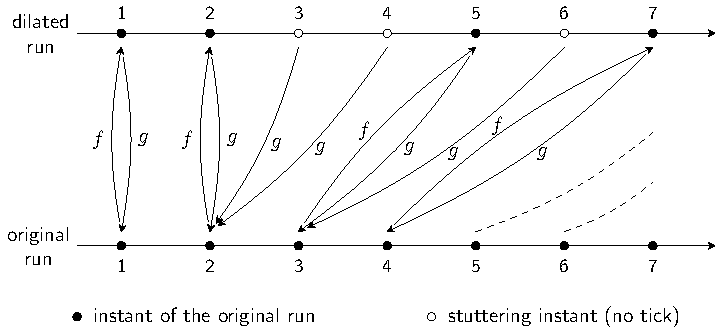
\includegraphics{dilating.pdf}
    \caption{Dilating and contracting functions}\label{fig:dilating-run}
  \end{figure}%
\end{isamarkuptext}\isamarkuptrue%
%
\begin{isamarkuptext}%
A function \isa{g} is contracting with respect to the dilation of run
\isa{sub} into run \isa{r} by the dilating function \isa{f} if:

%
\begin{itemize}%
\item it is a contracting function ;

\item \isa{{\isacharparenleft}f\ {\isasymcirc}\ g{\isacharparenright}\ n} is the index of the last original instant before instant 
\isa{n} in run \isa{r}, therefore:

%
\begin{itemize}%
\item \isa{{\isacharparenleft}f\ {\isasymcirc}\ g{\isacharparenright}\ n\ {\isasymle}\ n}

\item the time does not change on any clock between instants \isa{{\isacharparenleft}f\ {\isasymcirc}\ g{\isacharparenright}\ n}
and \isa{n} of run \isa{r};

\item no clock ticks before \isa{n} strictly after \isa{{\isacharparenleft}f\ {\isasymcirc}\ g{\isacharparenright}\ n} 
in run \isa{r}.
See \autoref{fig:dilating-run} for a better understanding. Notice that in this 
example, \isa{{\isadigit{2}}} is equal to \isa{{\isacharparenleft}f\ {\isasymcirc}\ g{\isacharparenright}\ {\isadigit{2}}}, \isa{{\isacharparenleft}f\ {\isasymcirc}\ g{\isacharparenright}\ {\isadigit{3}}}, 
and \isa{{\isacharparenleft}f\ {\isasymcirc}\ g{\isacharparenright}\ {\isadigit{4}}}. %
\end{itemize}%
\end{itemize}%
\end{isamarkuptext}\isamarkuptrue%
\isanewline
\isacommand{definition}\isamarkupfalse%
\ contracting\isanewline
\isakeyword{where}\ \isanewline
\ \ {\isacartoucheopen}contracting\ g\ r\ sub\ f\ {\isasymequiv}\ \ contracting{\isacharunderscore}fun\ g\isanewline
\ \ \ \ \ \ \ \ \ \ \ \ \ \ \ \ \ \ \ \ \ \ \ \ \ \ {\isasymand}\ {\isacharparenleft}{\isasymforall}n{\isachardot}\ f\ {\isacharparenleft}g\ n{\isacharparenright}\ {\isasymle}\ n{\isacharparenright}\isanewline
\ \ \ \ \ \ \ \ \ \ \ \ \ \ \ \ \ \ \ \ \ \ \ \ \ \ {\isasymand}\ {\isacharparenleft}{\isasymforall}n\ c\ k{\isachardot}\ f\ {\isacharparenleft}g\ n{\isacharparenright}\ {\isasymle}\ k\ {\isasymand}\ k\ {\isasymle}\ n\isanewline
\ \ \ \ \ \ \ \ \ \ \ \ \ \ \ \ \ \ \ \ \ \ \ \ \ \ \ \ \ \ {\isasymlongrightarrow}\ time\ {\isacharparenleft}{\isacharparenleft}Rep{\isacharunderscore}run\ r{\isacharparenright}\ k\ c{\isacharparenright}\ {\isacharequal}\ time\ {\isacharparenleft}{\isacharparenleft}Rep{\isacharunderscore}run\ sub{\isacharparenright}\ {\isacharparenleft}g\ n{\isacharparenright}\ c{\isacharparenright}{\isacharparenright}\isanewline
\ \ \ \ \ \ \ \ \ \ \ \ \ \ \ \ \ \ \ \ \ \ \ \ \ \ {\isasymand}\ {\isacharparenleft}{\isasymforall}n\ c\ k{\isachardot}\ f\ {\isacharparenleft}g\ n{\isacharparenright}\ {\isacharless}\ k\ {\isasymand}\ k\ {\isasymle}\ n\isanewline
\ \ \ \ \ \ \ \ \ \ \ \ \ \ \ \ \ \ \ \ \ \ \ \ \ \ \ \ \ \ {\isasymlongrightarrow}\ {\isasymnot}\ ticks\ {\isacharparenleft}{\isacharparenleft}Rep{\isacharunderscore}run\ r{\isacharparenright}\ k\ c{\isacharparenright}{\isacharparenright}{\isacartoucheclose}%
\begin{isamarkuptext}%
For any dilating function, we can build its \emph{inverse}, as illustrated on
  \autoref{fig:dilating-run}, which is a contracting function:%
\end{isamarkuptext}\isamarkuptrue%
\isacommand{definition}\isamarkupfalse%
\ {\isacartoucheopen}dil{\isacharunderscore}inverse\ f{\isacharcolon}{\isacharcolon}{\isacharparenleft}nat\ {\isasymRightarrow}\ nat{\isacharparenright}\ {\isasymequiv}\ {\isacharparenleft}{\isasymlambda}n{\isachardot}\ Max\ {\isacharbraceleft}i{\isachardot}\ f\ i\ {\isasymle}\ n{\isacharbraceright}{\isacharparenright}{\isacartoucheclose}%
\isadelimdocument
%
\endisadelimdocument
%
\isatagdocument
%
\isamarkupsubsection{Alternate definitions for counting ticks.%
}
\isamarkuptrue%
%
\endisatagdocument
{\isafolddocument}%
%
\isadelimdocument
%
\endisadelimdocument
%
\begin{isamarkuptext}%
For proving the stuttering invariance of TESL specifications, we will need
  these alternate definitions for counting ticks, which are based on sets.%
\end{isamarkuptext}\isamarkuptrue%
%
\begin{isamarkuptext}%
\isa{tick{\isacharunderscore}count\ r\ c\ n} is the number of ticks of clock \isa{c} in 
  run \isa{r} upto instant \isa{n}.%
\end{isamarkuptext}\isamarkuptrue%
\isacommand{definition}\isamarkupfalse%
\ tick{\isacharunderscore}count\ {\isacharcolon}{\isacharcolon}\ {\isacartoucheopen}{\isacharprime}a{\isacharcolon}{\isacharcolon}linordered{\isacharunderscore}field\ run\ {\isasymRightarrow}\ clock\ {\isasymRightarrow}\ nat\ {\isasymRightarrow}\ nat{\isacartoucheclose}\isanewline
\isakeyword{where}\isanewline
\ \ {\isacartoucheopen}tick{\isacharunderscore}count\ r\ c\ n\ {\isacharequal}\ card\ {\isacharbraceleft}i{\isachardot}\ i\ {\isasymle}\ n\ {\isasymand}\ ticks\ {\isacharparenleft}{\isacharparenleft}Rep{\isacharunderscore}run\ r{\isacharparenright}\ i\ c{\isacharparenright}{\isacharbraceright}{\isacartoucheclose}%
\begin{isamarkuptext}%
\isa{tick{\isacharunderscore}count{\isacharunderscore}strict\ r\ c\ n} is the number of ticks of clock \isa{c} 
  in run \isa{r} upto but excluding instant \isa{n}.%
\end{isamarkuptext}\isamarkuptrue%
\isacommand{definition}\isamarkupfalse%
\ tick{\isacharunderscore}count{\isacharunderscore}strict\ {\isacharcolon}{\isacharcolon}\ {\isacartoucheopen}{\isacharprime}a{\isacharcolon}{\isacharcolon}linordered{\isacharunderscore}field\ run\ {\isasymRightarrow}\ clock\ {\isasymRightarrow}\ nat\ {\isasymRightarrow}\ nat{\isacartoucheclose}\isanewline
\isakeyword{where}\isanewline
\ \ {\isacartoucheopen}tick{\isacharunderscore}count{\isacharunderscore}strict\ r\ c\ n\ {\isacharequal}\ card\ {\isacharbraceleft}i{\isachardot}\ i\ {\isacharless}\ n\ {\isasymand}\ ticks\ {\isacharparenleft}{\isacharparenleft}Rep{\isacharunderscore}run\ r{\isacharparenright}\ i\ c{\isacharparenright}{\isacharbraceright}{\isacartoucheclose}\isanewline
\isanewline
%
\isadelimtheory
\isanewline
%
\endisadelimtheory
%
\isatagtheory
\isacommand{end}\isamarkupfalse%
%
\endisatagtheory
{\isafoldtheory}%
%
\isadelimtheory
%
\endisadelimtheory
%
\end{isabellebody}%
\endinput
%:%file=~/MEGAsync/code/these/hygge/src/StutteringDefs.thy%:%
%:%11=1%:%
%:%15=3%:%
%:%31=5%:%
%:%32=5%:%
%:%33=6%:%
%:%34=7%:%
%:%35=8%:%
%:%36=9%:%
%:%45=12%:%
%:%46=13%:%
%:%47=14%:%
%:%48=15%:%
%:%49=16%:%
%:%58=19%:%
%:%70=22%:%
%:%71=23%:%
%:%72=24%:%
%:%73=25%:%
%:%74=26%:%
%:%78=27%:%
%:%80=28%:%
%:%81=29%:%
%:%83=30%:%
%:%84=31%:%
%:%86=32%:%
%:%87=33%:%
%:%90=35%:%
%:%91=35%:%
%:%92=36%:%
%:%93=37%:%
%:%100=45%:%
%:%101=46%:%
%:%105=47%:%
%:%107=48%:%
%:%109=49%:%
%:%112=51%:%
%:%113=51%:%
%:%114=52%:%
%:%115=53%:%
%:%119=58%:%
%:%121=60%:%
%:%122=60%:%
%:%123=61%:%
%:%124=62%:%
%:%126=65%:%
%:%127=66%:%
%:%128=67%:%
%:%129=68%:%
%:%130=69%:%
%:%131=70%:%
%:%132=71%:%
%:%134=73%:%
%:%135=73%:%
%:%136=74%:%
%:%138=77%:%
%:%139=78%:%
%:%140=79%:%
%:%141=80%:%
%:%142=81%:%
%:%143=82%:%
%:%144=83%:%
%:%145=84%:%
%:%149=96%:%
%:%150=97%:%
%:%154=98%:%
%:%156=99%:%
%:%157=100%:%
%:%163=102%:%
%:%164=103%:%
%:%166=104%:%
%:%167=105%:%
%:%168=106%:%
%:%169=107%:%
%:%170=108%:%
%:%174=115%:%
%:%175=116%:%
%:%176=116%:%
%:%177=117%:%
%:%178=118%:%
%:%185=126%:%
%:%186=127%:%
%:%188=129%:%
%:%189=129%:%
%:%196=132%:%
%:%208=135%:%
%:%209=136%:%
%:%213=140%:%
%:%214=141%:%
%:%216=143%:%
%:%217=143%:%
%:%218=144%:%
%:%219=145%:%
%:%221=148%:%
%:%222=149%:%
%:%224=151%:%
%:%225=151%:%
%:%226=152%:%
%:%227=153%:%
%:%228=154%:%
%:%231=155%:%
%:%236=156%:%